% Graphic for TeX using PGF
% Title: /home/anthony/Téléchargements/Realisation/Diagramme1.dia
% Creator: Dia v0.97.2
% CreationDate: Thu Mar 13 11:20:15 2014
% For: anthony
% \usepackage{tikz}
% The following commands are not supported in PSTricks at present
% We define them conditionally, so when they are implemented,
% this pgf file will use them.
\ifx\du\undefined
  \newlength{\du}
\fi
\setlength{\du}{15\unitlength}
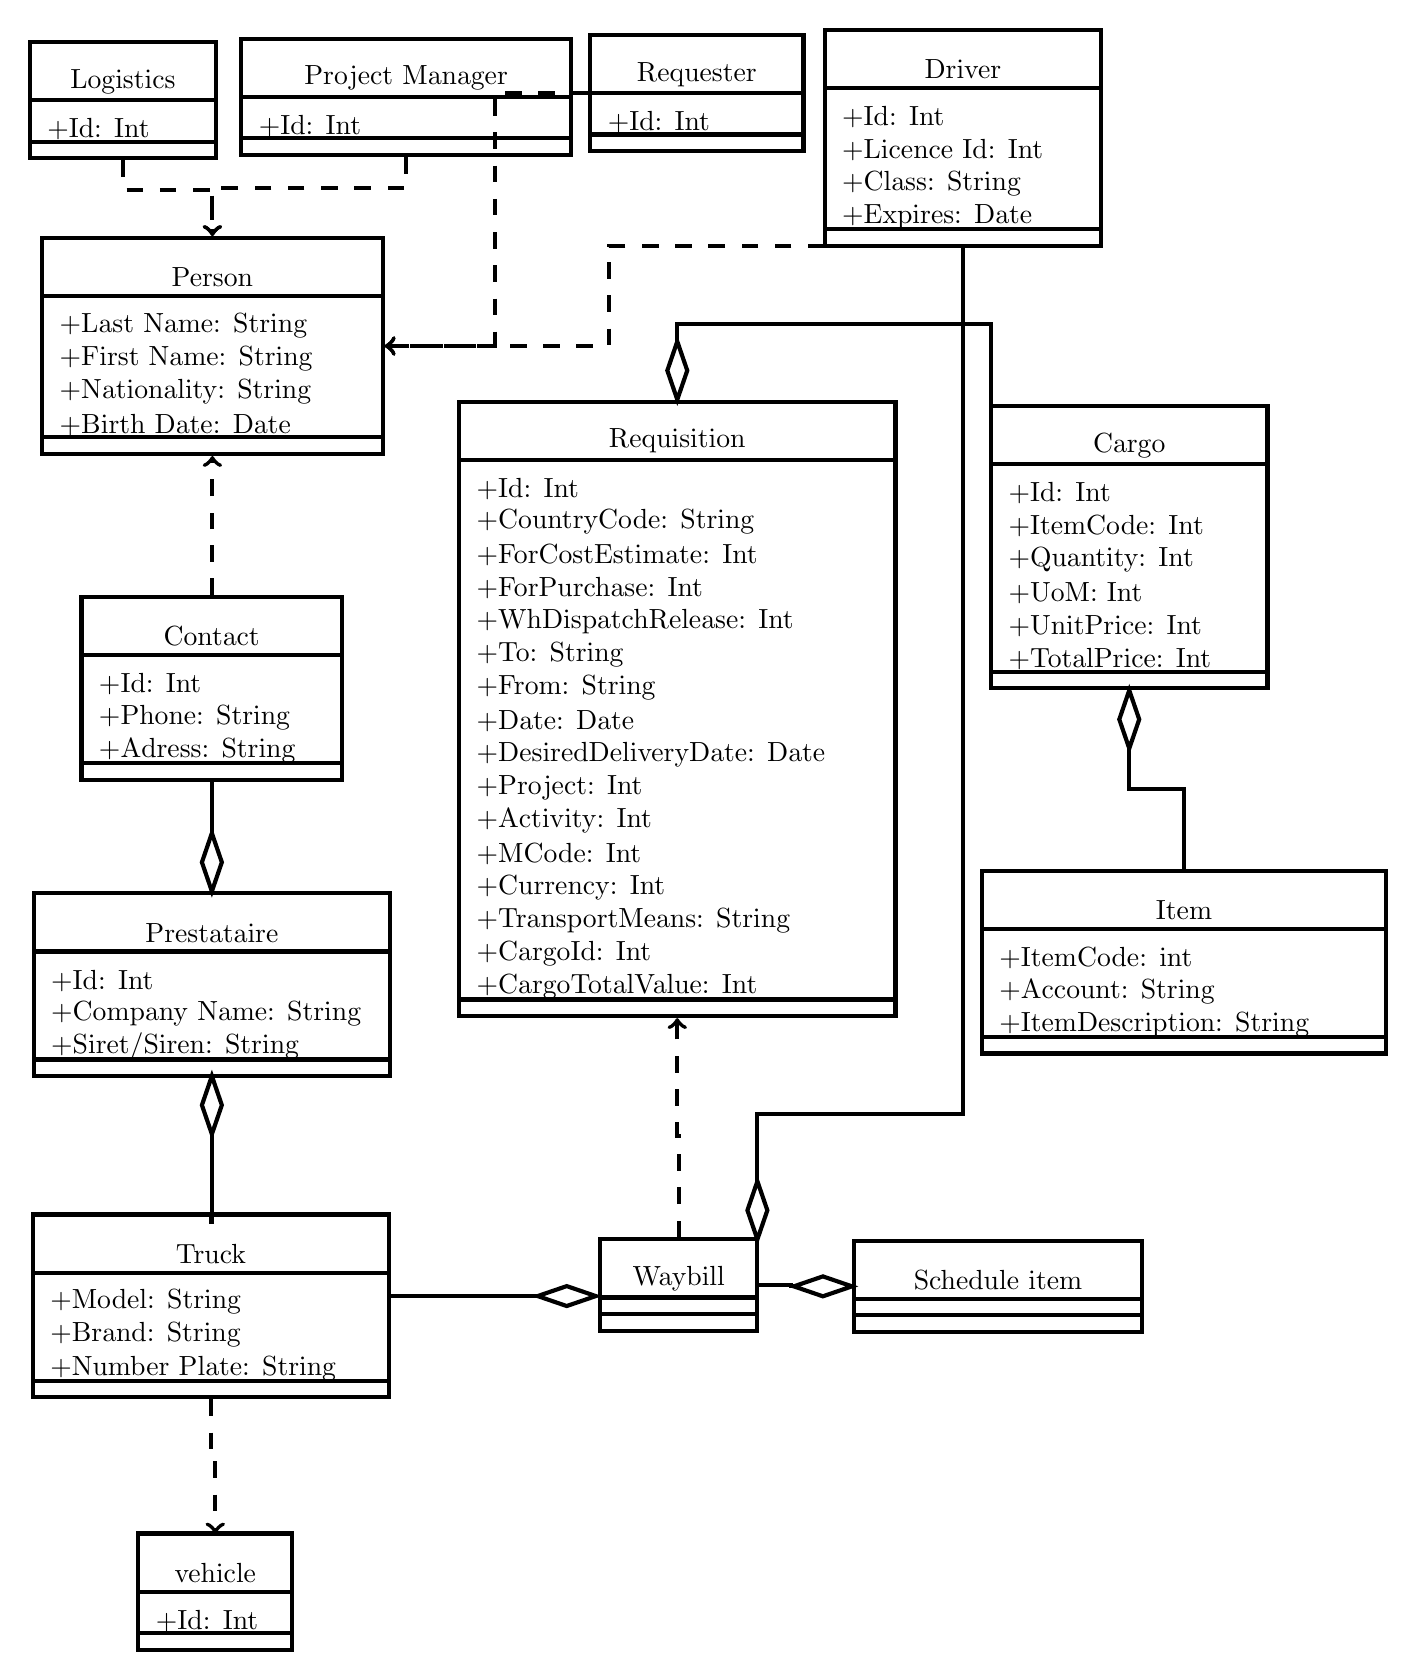
\begin{tikzpicture}
\pgftransformxscale{1.000000}
\pgftransformyscale{-1.000000}
\definecolor{dialinecolor}{rgb}{0.000000, 0.000000, 0.000000}
\pgfsetstrokecolor{dialinecolor}
\definecolor{dialinecolor}{rgb}{1.000000, 1.000000, 1.000000}
\pgfsetfillcolor{dialinecolor}
\pgfsetlinewidth{0.100000\du}
\pgfsetdash{}{0pt}
\definecolor{dialinecolor}{rgb}{1.000000, 1.000000, 1.000000}
\pgfsetfillcolor{dialinecolor}
\fill (0.627412\du,4.970013\du)--(0.627412\du,6.370013\du)--(8.827412\du,6.370013\du)--(8.827412\du,4.970013\du)--cycle;
\definecolor{dialinecolor}{rgb}{0.000000, 0.000000, 0.000000}
\pgfsetstrokecolor{dialinecolor}
\draw (0.627412\du,4.970013\du)--(0.627412\du,6.370013\du)--(8.827412\du,6.370013\du)--(8.827412\du,4.970013\du)--cycle;
% setfont left to latex
\definecolor{dialinecolor}{rgb}{0.000000, 0.000000, 0.000000}
\pgfsetstrokecolor{dialinecolor}
\node at (4.727412\du,5.920013\du){Person};
\definecolor{dialinecolor}{rgb}{1.000000, 1.000000, 1.000000}
\pgfsetfillcolor{dialinecolor}
\fill (0.627412\du,6.370013\du)--(0.627412\du,9.770013\du)--(8.827412\du,9.770013\du)--(8.827412\du,6.370013\du)--cycle;
\definecolor{dialinecolor}{rgb}{0.000000, 0.000000, 0.000000}
\pgfsetstrokecolor{dialinecolor}
\draw (0.627412\du,6.370013\du)--(0.627412\du,9.770013\du)--(8.827412\du,9.770013\du)--(8.827412\du,6.370013\du)--cycle;
% setfont left to latex
\definecolor{dialinecolor}{rgb}{0.000000, 0.000000, 0.000000}
\pgfsetstrokecolor{dialinecolor}
\node[anchor=west] at (0.777412\du,7.070013\du){+Last Name: String};
% setfont left to latex
\definecolor{dialinecolor}{rgb}{0.000000, 0.000000, 0.000000}
\pgfsetstrokecolor{dialinecolor}
\node[anchor=west] at (0.777412\du,7.870013\du){+First Name: String};
% setfont left to latex
\definecolor{dialinecolor}{rgb}{0.000000, 0.000000, 0.000000}
\pgfsetstrokecolor{dialinecolor}
\node[anchor=west] at (0.777412\du,8.670013\du){+Nationality: String};
% setfont left to latex
\definecolor{dialinecolor}{rgb}{0.000000, 0.000000, 0.000000}
\pgfsetstrokecolor{dialinecolor}
\node[anchor=west] at (0.777412\du,9.470013\du){+Birth Date: Date};
\definecolor{dialinecolor}{rgb}{1.000000, 1.000000, 1.000000}
\pgfsetfillcolor{dialinecolor}
\fill (0.627412\du,9.770013\du)--(0.627412\du,10.170013\du)--(8.827412\du,10.170013\du)--(8.827412\du,9.770013\du)--cycle;
\definecolor{dialinecolor}{rgb}{0.000000, 0.000000, 0.000000}
\pgfsetstrokecolor{dialinecolor}
\draw (0.627412\du,9.770013\du)--(0.627412\du,10.170013\du)--(8.827412\du,10.170013\du)--(8.827412\du,9.770013\du)--cycle;
\pgfsetlinewidth{0.100000\du}
\pgfsetdash{}{0pt}
\definecolor{dialinecolor}{rgb}{1.000000, 1.000000, 1.000000}
\pgfsetfillcolor{dialinecolor}
\fill (19.476165\du,-0.048711\du)--(19.476165\du,1.351289\du)--(26.136165\du,1.351289\du)--(26.136165\du,-0.048711\du)--cycle;
\definecolor{dialinecolor}{rgb}{0.000000, 0.000000, 0.000000}
\pgfsetstrokecolor{dialinecolor}
\draw (19.476165\du,-0.048711\du)--(19.476165\du,1.351289\du)--(26.136165\du,1.351289\du)--(26.136165\du,-0.048711\du)--cycle;
% setfont left to latex
\definecolor{dialinecolor}{rgb}{0.000000, 0.000000, 0.000000}
\pgfsetstrokecolor{dialinecolor}
\node at (22.806165\du,0.901289\du){Driver};
\definecolor{dialinecolor}{rgb}{1.000000, 1.000000, 1.000000}
\pgfsetfillcolor{dialinecolor}
\fill (19.476165\du,1.351289\du)--(19.476165\du,4.751289\du)--(26.136165\du,4.751289\du)--(26.136165\du,1.351289\du)--cycle;
\definecolor{dialinecolor}{rgb}{0.000000, 0.000000, 0.000000}
\pgfsetstrokecolor{dialinecolor}
\draw (19.476165\du,1.351289\du)--(19.476165\du,4.751289\du)--(26.136165\du,4.751289\du)--(26.136165\du,1.351289\du)--cycle;
% setfont left to latex
\definecolor{dialinecolor}{rgb}{0.000000, 0.000000, 0.000000}
\pgfsetstrokecolor{dialinecolor}
\node[anchor=west] at (19.626165\du,2.051289\du){+Id: Int};
% setfont left to latex
\definecolor{dialinecolor}{rgb}{0.000000, 0.000000, 0.000000}
\pgfsetstrokecolor{dialinecolor}
\node[anchor=west] at (19.626165\du,2.851289\du){+Licence Id: Int};
% setfont left to latex
\definecolor{dialinecolor}{rgb}{0.000000, 0.000000, 0.000000}
\pgfsetstrokecolor{dialinecolor}
\node[anchor=west] at (19.626165\du,3.651289\du){+Class: String};
% setfont left to latex
\definecolor{dialinecolor}{rgb}{0.000000, 0.000000, 0.000000}
\pgfsetstrokecolor{dialinecolor}
\node[anchor=west] at (19.626165\du,4.451289\du){+Expires: Date};
\definecolor{dialinecolor}{rgb}{1.000000, 1.000000, 1.000000}
\pgfsetfillcolor{dialinecolor}
\fill (19.476165\du,4.751289\du)--(19.476165\du,5.151289\du)--(26.136165\du,5.151289\du)--(26.136165\du,4.751289\du)--cycle;
\definecolor{dialinecolor}{rgb}{0.000000, 0.000000, 0.000000}
\pgfsetstrokecolor{dialinecolor}
\draw (19.476165\du,4.751289\du)--(19.476165\du,5.151289\du)--(26.136165\du,5.151289\du)--(26.136165\du,4.751289\du)--cycle;
\pgfsetlinewidth{0.100000\du}
\pgfsetdash{}{0pt}
\definecolor{dialinecolor}{rgb}{1.000000, 1.000000, 1.000000}
\pgfsetfillcolor{dialinecolor}
\fill (2.945199\du,36.175328\du)--(2.945199\du,37.575328\du)--(6.647699\du,37.575328\du)--(6.647699\du,36.175328\du)--cycle;
\definecolor{dialinecolor}{rgb}{0.000000, 0.000000, 0.000000}
\pgfsetstrokecolor{dialinecolor}
\draw (2.945199\du,36.175328\du)--(2.945199\du,37.575328\du)--(6.647699\du,37.575328\du)--(6.647699\du,36.175328\du)--cycle;
% setfont left to latex
\definecolor{dialinecolor}{rgb}{0.000000, 0.000000, 0.000000}
\pgfsetstrokecolor{dialinecolor}
\node at (4.796449\du,37.125328\du){vehicle};
\definecolor{dialinecolor}{rgb}{1.000000, 1.000000, 1.000000}
\pgfsetfillcolor{dialinecolor}
\fill (2.945199\du,37.575328\du)--(2.945199\du,38.575328\du)--(6.647699\du,38.575328\du)--(6.647699\du,37.575328\du)--cycle;
\definecolor{dialinecolor}{rgb}{0.000000, 0.000000, 0.000000}
\pgfsetstrokecolor{dialinecolor}
\draw (2.945199\du,37.575328\du)--(2.945199\du,38.575328\du)--(6.647699\du,38.575328\du)--(6.647699\du,37.575328\du)--cycle;
% setfont left to latex
\definecolor{dialinecolor}{rgb}{0.000000, 0.000000, 0.000000}
\pgfsetstrokecolor{dialinecolor}
\node[anchor=west] at (3.095199\du,38.275328\du){+Id: Int};
\definecolor{dialinecolor}{rgb}{1.000000, 1.000000, 1.000000}
\pgfsetfillcolor{dialinecolor}
\fill (2.945199\du,38.575328\du)--(2.945199\du,38.975328\du)--(6.647699\du,38.975328\du)--(6.647699\du,38.575328\du)--cycle;
\definecolor{dialinecolor}{rgb}{0.000000, 0.000000, 0.000000}
\pgfsetstrokecolor{dialinecolor}
\draw (2.945199\du,38.575328\du)--(2.945199\du,38.975328\du)--(6.647699\du,38.975328\du)--(6.647699\du,38.575328\du)--cycle;
\pgfsetlinewidth{0.100000\du}
\pgfsetdash{}{0pt}
\definecolor{dialinecolor}{rgb}{1.000000, 1.000000, 1.000000}
\pgfsetfillcolor{dialinecolor}
\fill (0.400279\du,28.492925\du)--(0.400279\du,29.892925\du)--(8.985279\du,29.892925\du)--(8.985279\du,28.492925\du)--cycle;
\definecolor{dialinecolor}{rgb}{0.000000, 0.000000, 0.000000}
\pgfsetstrokecolor{dialinecolor}
\draw (0.400279\du,28.492925\du)--(0.400279\du,29.892925\du)--(8.985279\du,29.892925\du)--(8.985279\du,28.492925\du)--cycle;
% setfont left to latex
\definecolor{dialinecolor}{rgb}{0.000000, 0.000000, 0.000000}
\pgfsetstrokecolor{dialinecolor}
\node at (4.692779\du,29.442925\du){Truck};
\definecolor{dialinecolor}{rgb}{1.000000, 1.000000, 1.000000}
\pgfsetfillcolor{dialinecolor}
\fill (0.400279\du,29.892925\du)--(0.400279\du,32.492925\du)--(8.985279\du,32.492925\du)--(8.985279\du,29.892925\du)--cycle;
\definecolor{dialinecolor}{rgb}{0.000000, 0.000000, 0.000000}
\pgfsetstrokecolor{dialinecolor}
\draw (0.400279\du,29.892925\du)--(0.400279\du,32.492925\du)--(8.985279\du,32.492925\du)--(8.985279\du,29.892925\du)--cycle;
% setfont left to latex
\definecolor{dialinecolor}{rgb}{0.000000, 0.000000, 0.000000}
\pgfsetstrokecolor{dialinecolor}
\node[anchor=west] at (0.550279\du,30.592925\du){+Model: String};
% setfont left to latex
\definecolor{dialinecolor}{rgb}{0.000000, 0.000000, 0.000000}
\pgfsetstrokecolor{dialinecolor}
\node[anchor=west] at (0.550279\du,31.392925\du){+Brand: String};
% setfont left to latex
\definecolor{dialinecolor}{rgb}{0.000000, 0.000000, 0.000000}
\pgfsetstrokecolor{dialinecolor}
\node[anchor=west] at (0.550279\du,32.192925\du){+Number Plate: String};
\definecolor{dialinecolor}{rgb}{1.000000, 1.000000, 1.000000}
\pgfsetfillcolor{dialinecolor}
\fill (0.400279\du,32.492925\du)--(0.400279\du,32.892925\du)--(8.985279\du,32.892925\du)--(8.985279\du,32.492925\du)--cycle;
\definecolor{dialinecolor}{rgb}{0.000000, 0.000000, 0.000000}
\pgfsetstrokecolor{dialinecolor}
\draw (0.400279\du,32.492925\du)--(0.400279\du,32.892925\du)--(8.985279\du,32.892925\du)--(8.985279\du,32.492925\du)--cycle;
\pgfsetlinewidth{0.100000\du}
\pgfsetdash{}{0pt}
\definecolor{dialinecolor}{rgb}{1.000000, 1.000000, 1.000000}
\pgfsetfillcolor{dialinecolor}
\fill (0.422512\du,20.756413\du)--(0.422512\du,22.156413\du)--(9.007512\du,22.156413\du)--(9.007512\du,20.756413\du)--cycle;
\definecolor{dialinecolor}{rgb}{0.000000, 0.000000, 0.000000}
\pgfsetstrokecolor{dialinecolor}
\draw (0.422512\du,20.756413\du)--(0.422512\du,22.156413\du)--(9.007512\du,22.156413\du)--(9.007512\du,20.756413\du)--cycle;
% setfont left to latex
\definecolor{dialinecolor}{rgb}{0.000000, 0.000000, 0.000000}
\pgfsetstrokecolor{dialinecolor}
\node at (4.715012\du,21.706413\du){Prestataire};
\definecolor{dialinecolor}{rgb}{1.000000, 1.000000, 1.000000}
\pgfsetfillcolor{dialinecolor}
\fill (0.422512\du,22.156413\du)--(0.422512\du,24.756413\du)--(9.007512\du,24.756413\du)--(9.007512\du,22.156413\du)--cycle;
\definecolor{dialinecolor}{rgb}{0.000000, 0.000000, 0.000000}
\pgfsetstrokecolor{dialinecolor}
\draw (0.422512\du,22.156413\du)--(0.422512\du,24.756413\du)--(9.007512\du,24.756413\du)--(9.007512\du,22.156413\du)--cycle;
% setfont left to latex
\definecolor{dialinecolor}{rgb}{0.000000, 0.000000, 0.000000}
\pgfsetstrokecolor{dialinecolor}
\node[anchor=west] at (0.572512\du,22.856413\du){+Id: Int};
% setfont left to latex
\definecolor{dialinecolor}{rgb}{0.000000, 0.000000, 0.000000}
\pgfsetstrokecolor{dialinecolor}
\node[anchor=west] at (0.572512\du,23.656413\du){+Company Name: String};
% setfont left to latex
\definecolor{dialinecolor}{rgb}{0.000000, 0.000000, 0.000000}
\pgfsetstrokecolor{dialinecolor}
\node[anchor=west] at (0.572512\du,24.456413\du){+Siret/Siren: String};
\definecolor{dialinecolor}{rgb}{1.000000, 1.000000, 1.000000}
\pgfsetfillcolor{dialinecolor}
\fill (0.422512\du,24.756413\du)--(0.422512\du,25.156413\du)--(9.007512\du,25.156413\du)--(9.007512\du,24.756413\du)--cycle;
\definecolor{dialinecolor}{rgb}{0.000000, 0.000000, 0.000000}
\pgfsetstrokecolor{dialinecolor}
\draw (0.422512\du,24.756413\du)--(0.422512\du,25.156413\du)--(9.007512\du,25.156413\du)--(9.007512\du,24.756413\du)--cycle;
\pgfsetlinewidth{0.100000\du}
\pgfsetdash{}{0pt}
\definecolor{dialinecolor}{rgb}{1.000000, 1.000000, 1.000000}
\pgfsetfillcolor{dialinecolor}
\fill (1.573212\du,13.617397\du)--(1.573212\du,15.017397\du)--(7.848212\du,15.017397\du)--(7.848212\du,13.617397\du)--cycle;
\definecolor{dialinecolor}{rgb}{0.000000, 0.000000, 0.000000}
\pgfsetstrokecolor{dialinecolor}
\draw (1.573212\du,13.617397\du)--(1.573212\du,15.017397\du)--(7.848212\du,15.017397\du)--(7.848212\du,13.617397\du)--cycle;
% setfont left to latex
\definecolor{dialinecolor}{rgb}{0.000000, 0.000000, 0.000000}
\pgfsetstrokecolor{dialinecolor}
\node at (4.710712\du,14.567397\du){Contact};
\definecolor{dialinecolor}{rgb}{1.000000, 1.000000, 1.000000}
\pgfsetfillcolor{dialinecolor}
\fill (1.573212\du,15.017397\du)--(1.573212\du,17.617397\du)--(7.848212\du,17.617397\du)--(7.848212\du,15.017397\du)--cycle;
\definecolor{dialinecolor}{rgb}{0.000000, 0.000000, 0.000000}
\pgfsetstrokecolor{dialinecolor}
\draw (1.573212\du,15.017397\du)--(1.573212\du,17.617397\du)--(7.848212\du,17.617397\du)--(7.848212\du,15.017397\du)--cycle;
% setfont left to latex
\definecolor{dialinecolor}{rgb}{0.000000, 0.000000, 0.000000}
\pgfsetstrokecolor{dialinecolor}
\node[anchor=west] at (1.723212\du,15.717397\du){+Id: Int};
% setfont left to latex
\definecolor{dialinecolor}{rgb}{0.000000, 0.000000, 0.000000}
\pgfsetstrokecolor{dialinecolor}
\node[anchor=west] at (1.723212\du,16.517397\du){+Phone: String};
% setfont left to latex
\definecolor{dialinecolor}{rgb}{0.000000, 0.000000, 0.000000}
\pgfsetstrokecolor{dialinecolor}
\node[anchor=west] at (1.723212\du,17.317397\du){+Adress: String};
\definecolor{dialinecolor}{rgb}{1.000000, 1.000000, 1.000000}
\pgfsetfillcolor{dialinecolor}
\fill (1.573212\du,17.617397\du)--(1.573212\du,18.017397\du)--(7.848212\du,18.017397\du)--(7.848212\du,17.617397\du)--cycle;
\definecolor{dialinecolor}{rgb}{0.000000, 0.000000, 0.000000}
\pgfsetstrokecolor{dialinecolor}
\draw (1.573212\du,17.617397\du)--(1.573212\du,18.017397\du)--(7.848212\du,18.017397\du)--(7.848212\du,17.617397\du)--cycle;
\pgfsetlinewidth{0.100000\du}
\pgfsetdash{}{0pt}
\definecolor{dialinecolor}{rgb}{1.000000, 1.000000, 1.000000}
\pgfsetfillcolor{dialinecolor}
\fill (10.671605\du,8.910942\du)--(10.671605\du,10.310942\du)--(21.181605\du,10.310942\du)--(21.181605\du,8.910942\du)--cycle;
\definecolor{dialinecolor}{rgb}{0.000000, 0.000000, 0.000000}
\pgfsetstrokecolor{dialinecolor}
\draw (10.671605\du,8.910942\du)--(10.671605\du,10.310942\du)--(21.181605\du,10.310942\du)--(21.181605\du,8.910942\du)--cycle;
% setfont left to latex
\definecolor{dialinecolor}{rgb}{0.000000, 0.000000, 0.000000}
\pgfsetstrokecolor{dialinecolor}
\node at (15.926605\du,9.860942\du){Requisition};
\definecolor{dialinecolor}{rgb}{1.000000, 1.000000, 1.000000}
\pgfsetfillcolor{dialinecolor}
\fill (10.671605\du,10.310942\du)--(10.671605\du,23.310942\du)--(21.181605\du,23.310942\du)--(21.181605\du,10.310942\du)--cycle;
\definecolor{dialinecolor}{rgb}{0.000000, 0.000000, 0.000000}
\pgfsetstrokecolor{dialinecolor}
\draw (10.671605\du,10.310942\du)--(10.671605\du,23.310942\du)--(21.181605\du,23.310942\du)--(21.181605\du,10.310942\du)--cycle;
% setfont left to latex
\definecolor{dialinecolor}{rgb}{0.000000, 0.000000, 0.000000}
\pgfsetstrokecolor{dialinecolor}
\node[anchor=west] at (10.821605\du,11.010942\du){+Id: Int};
% setfont left to latex
\definecolor{dialinecolor}{rgb}{0.000000, 0.000000, 0.000000}
\pgfsetstrokecolor{dialinecolor}
\node[anchor=west] at (10.821605\du,11.810942\du){+CountryCode: String};
% setfont left to latex
\definecolor{dialinecolor}{rgb}{0.000000, 0.000000, 0.000000}
\pgfsetstrokecolor{dialinecolor}
\node[anchor=west] at (10.821605\du,12.610942\du){+ForCostEstimate: Int};
% setfont left to latex
\definecolor{dialinecolor}{rgb}{0.000000, 0.000000, 0.000000}
\pgfsetstrokecolor{dialinecolor}
\node[anchor=west] at (10.821605\du,13.410942\du){+ForPurchase: Int};
% setfont left to latex
\definecolor{dialinecolor}{rgb}{0.000000, 0.000000, 0.000000}
\pgfsetstrokecolor{dialinecolor}
\node[anchor=west] at (10.821605\du,14.210942\du){+WhDispatchRelease: Int};
% setfont left to latex
\definecolor{dialinecolor}{rgb}{0.000000, 0.000000, 0.000000}
\pgfsetstrokecolor{dialinecolor}
\node[anchor=west] at (10.821605\du,15.010942\du){+To: String};
% setfont left to latex
\definecolor{dialinecolor}{rgb}{0.000000, 0.000000, 0.000000}
\pgfsetstrokecolor{dialinecolor}
\node[anchor=west] at (10.821605\du,15.810942\du){+From: String};
% setfont left to latex
\definecolor{dialinecolor}{rgb}{0.000000, 0.000000, 0.000000}
\pgfsetstrokecolor{dialinecolor}
\node[anchor=west] at (10.821605\du,16.610942\du){+Date: Date};
% setfont left to latex
\definecolor{dialinecolor}{rgb}{0.000000, 0.000000, 0.000000}
\pgfsetstrokecolor{dialinecolor}
\node[anchor=west] at (10.821605\du,17.410942\du){+DesiredDeliveryDate: Date};
% setfont left to latex
\definecolor{dialinecolor}{rgb}{0.000000, 0.000000, 0.000000}
\pgfsetstrokecolor{dialinecolor}
\node[anchor=west] at (10.821605\du,18.210942\du){+Project: Int};
% setfont left to latex
\definecolor{dialinecolor}{rgb}{0.000000, 0.000000, 0.000000}
\pgfsetstrokecolor{dialinecolor}
\node[anchor=west] at (10.821605\du,19.010942\du){+Activity: Int};
% setfont left to latex
\definecolor{dialinecolor}{rgb}{0.000000, 0.000000, 0.000000}
\pgfsetstrokecolor{dialinecolor}
\node[anchor=west] at (10.821605\du,19.810942\du){+MCode: Int};
% setfont left to latex
\definecolor{dialinecolor}{rgb}{0.000000, 0.000000, 0.000000}
\pgfsetstrokecolor{dialinecolor}
\node[anchor=west] at (10.821605\du,20.610942\du){+Currency: Int};
% setfont left to latex
\definecolor{dialinecolor}{rgb}{0.000000, 0.000000, 0.000000}
\pgfsetstrokecolor{dialinecolor}
\node[anchor=west] at (10.821605\du,21.410942\du){+TransportMeans: String};
% setfont left to latex
\definecolor{dialinecolor}{rgb}{0.000000, 0.000000, 0.000000}
\pgfsetstrokecolor{dialinecolor}
\node[anchor=west] at (10.821605\du,22.210942\du){+CargoId: Int};
% setfont left to latex
\definecolor{dialinecolor}{rgb}{0.000000, 0.000000, 0.000000}
\pgfsetstrokecolor{dialinecolor}
\node[anchor=west] at (10.821605\du,23.010942\du){+CargoTotalValue: Int};
\definecolor{dialinecolor}{rgb}{1.000000, 1.000000, 1.000000}
\pgfsetfillcolor{dialinecolor}
\fill (10.671605\du,23.310942\du)--(10.671605\du,23.710942\du)--(21.181605\du,23.710942\du)--(21.181605\du,23.310942\du)--cycle;
\definecolor{dialinecolor}{rgb}{0.000000, 0.000000, 0.000000}
\pgfsetstrokecolor{dialinecolor}
\draw (10.671605\du,23.310942\du)--(10.671605\du,23.710942\du)--(21.181605\du,23.710942\du)--(21.181605\du,23.310942\du)--cycle;
\pgfsetlinewidth{0.100000\du}
\pgfsetdash{}{0pt}
\definecolor{dialinecolor}{rgb}{1.000000, 1.000000, 1.000000}
\pgfsetfillcolor{dialinecolor}
\fill (20.184950\du,29.122676\du)--(20.184950\du,30.522676\du)--(27.117450\du,30.522676\du)--(27.117450\du,29.122676\du)--cycle;
\definecolor{dialinecolor}{rgb}{0.000000, 0.000000, 0.000000}
\pgfsetstrokecolor{dialinecolor}
\draw (20.184950\du,29.122676\du)--(20.184950\du,30.522676\du)--(27.117450\du,30.522676\du)--(27.117450\du,29.122676\du)--cycle;
% setfont left to latex
\definecolor{dialinecolor}{rgb}{0.000000, 0.000000, 0.000000}
\pgfsetstrokecolor{dialinecolor}
\node at (23.651200\du,30.072676\du){Schedule item};
\definecolor{dialinecolor}{rgb}{1.000000, 1.000000, 1.000000}
\pgfsetfillcolor{dialinecolor}
\fill (20.184950\du,30.522676\du)--(20.184950\du,30.922676\du)--(27.117450\du,30.922676\du)--(27.117450\du,30.522676\du)--cycle;
\definecolor{dialinecolor}{rgb}{0.000000, 0.000000, 0.000000}
\pgfsetstrokecolor{dialinecolor}
\draw (20.184950\du,30.522676\du)--(20.184950\du,30.922676\du)--(27.117450\du,30.922676\du)--(27.117450\du,30.522676\du)--cycle;
\definecolor{dialinecolor}{rgb}{1.000000, 1.000000, 1.000000}
\pgfsetfillcolor{dialinecolor}
\fill (20.184950\du,30.922676\du)--(20.184950\du,31.322676\du)--(27.117450\du,31.322676\du)--(27.117450\du,30.922676\du)--cycle;
\definecolor{dialinecolor}{rgb}{0.000000, 0.000000, 0.000000}
\pgfsetstrokecolor{dialinecolor}
\draw (20.184950\du,30.922676\du)--(20.184950\du,31.322676\du)--(27.117450\du,31.322676\du)--(27.117450\du,30.922676\du)--cycle;
\pgfsetlinewidth{0.100000\du}
\pgfsetdash{}{0pt}
\definecolor{dialinecolor}{rgb}{1.000000, 1.000000, 1.000000}
\pgfsetfillcolor{dialinecolor}
\fill (23.484568\du,9.014023\du)--(23.484568\du,10.414023\du)--(30.144568\du,10.414023\du)--(30.144568\du,9.014023\du)--cycle;
\definecolor{dialinecolor}{rgb}{0.000000, 0.000000, 0.000000}
\pgfsetstrokecolor{dialinecolor}
\draw (23.484568\du,9.014023\du)--(23.484568\du,10.414023\du)--(30.144568\du,10.414023\du)--(30.144568\du,9.014023\du)--cycle;
% setfont left to latex
\definecolor{dialinecolor}{rgb}{0.000000, 0.000000, 0.000000}
\pgfsetstrokecolor{dialinecolor}
\node at (26.814568\du,9.964023\du){Cargo};
\definecolor{dialinecolor}{rgb}{1.000000, 1.000000, 1.000000}
\pgfsetfillcolor{dialinecolor}
\fill (23.484568\du,10.414023\du)--(23.484568\du,15.414023\du)--(30.144568\du,15.414023\du)--(30.144568\du,10.414023\du)--cycle;
\definecolor{dialinecolor}{rgb}{0.000000, 0.000000, 0.000000}
\pgfsetstrokecolor{dialinecolor}
\draw (23.484568\du,10.414023\du)--(23.484568\du,15.414023\du)--(30.144568\du,15.414023\du)--(30.144568\du,10.414023\du)--cycle;
% setfont left to latex
\definecolor{dialinecolor}{rgb}{0.000000, 0.000000, 0.000000}
\pgfsetstrokecolor{dialinecolor}
\node[anchor=west] at (23.634568\du,11.114023\du){+Id: Int};
% setfont left to latex
\definecolor{dialinecolor}{rgb}{0.000000, 0.000000, 0.000000}
\pgfsetstrokecolor{dialinecolor}
\node[anchor=west] at (23.634568\du,11.914023\du){+ItemCode: Int};
% setfont left to latex
\definecolor{dialinecolor}{rgb}{0.000000, 0.000000, 0.000000}
\pgfsetstrokecolor{dialinecolor}
\node[anchor=west] at (23.634568\du,12.714023\du){+Quantity: Int};
% setfont left to latex
\definecolor{dialinecolor}{rgb}{0.000000, 0.000000, 0.000000}
\pgfsetstrokecolor{dialinecolor}
\node[anchor=west] at (23.634568\du,13.514023\du){+UoM: Int};
% setfont left to latex
\definecolor{dialinecolor}{rgb}{0.000000, 0.000000, 0.000000}
\pgfsetstrokecolor{dialinecolor}
\node[anchor=west] at (23.634568\du,14.314023\du){+UnitPrice: Int};
% setfont left to latex
\definecolor{dialinecolor}{rgb}{0.000000, 0.000000, 0.000000}
\pgfsetstrokecolor{dialinecolor}
\node[anchor=west] at (23.634568\du,15.114023\du){+TotalPrice: Int};
\definecolor{dialinecolor}{rgb}{1.000000, 1.000000, 1.000000}
\pgfsetfillcolor{dialinecolor}
\fill (23.484568\du,15.414023\du)--(23.484568\du,15.814023\du)--(30.144568\du,15.814023\du)--(30.144568\du,15.414023\du)--cycle;
\definecolor{dialinecolor}{rgb}{0.000000, 0.000000, 0.000000}
\pgfsetstrokecolor{dialinecolor}
\draw (23.484568\du,15.414023\du)--(23.484568\du,15.814023\du)--(30.144568\du,15.814023\du)--(30.144568\du,15.414023\du)--cycle;
\pgfsetlinewidth{0.100000\du}
\pgfsetdash{{1.000000\du}{1.000000\du}}{0\du}
\pgfsetdash{{0.400000\du}{0.400000\du}}{0\du}
\pgfsetmiterjoin
\pgfsetbuttcap
{
\definecolor{dialinecolor}{rgb}{0.000000, 0.000000, 0.000000}
\pgfsetfillcolor{dialinecolor}
% was here!!!
\pgfsetarrowsend{to}
\definecolor{dialinecolor}{rgb}{0.000000, 0.000000, 0.000000}
\pgfsetstrokecolor{dialinecolor}
\draw (4.692779\du,32.943200\du)--(4.692779\du,34.359264\du)--(4.796449\du,34.359264\du)--(4.796449\du,36.175328\du);
}
% setfont left to latex
\pgfsetlinewidth{0.100000\du}
\pgfsetdash{}{0pt}
\pgfsetmiterjoin
\pgfsetbuttcap
{
\definecolor{dialinecolor}{rgb}{0.000000, 0.000000, 0.000000}
\pgfsetfillcolor{dialinecolor}
% was here!!!
\definecolor{dialinecolor}{rgb}{0.000000, 0.000000, 0.000000}
\pgfsetstrokecolor{dialinecolor}
\draw (4.715012\du,25.156413\du)--(4.715012\du,28.665070\du)--(4.692779\du,28.665070\du)--(4.692779\du,28.492925\du);
}
\definecolor{dialinecolor}{rgb}{0.000000, 0.000000, 0.000000}
\pgfsetstrokecolor{dialinecolor}
\draw (4.715012\du,26.414991\du)--(4.715012\du,28.665070\du)--(4.692779\du,28.665070\du)--(4.692779\du,28.492925\du);
\pgfsetdash{}{0pt}
\pgfsetmiterjoin
\pgfsetbuttcap
\definecolor{dialinecolor}{rgb}{1.000000, 1.000000, 1.000000}
\pgfsetfillcolor{dialinecolor}
\fill (4.715012\du,25.156413\du)--(4.955012\du,25.856413\du)--(4.715012\du,26.556413\du)--(4.475012\du,25.856413\du)--cycle;
\pgfsetlinewidth{0.100000\du}
\pgfsetdash{}{0pt}
\pgfsetmiterjoin
\pgfsetbuttcap
\definecolor{dialinecolor}{rgb}{0.000000, 0.000000, 0.000000}
\pgfsetstrokecolor{dialinecolor}
\draw (4.715012\du,25.156413\du)--(4.955012\du,25.856413\du)--(4.715012\du,26.556413\du)--(4.475012\du,25.856413\du)--cycle;
% setfont left to latex
\definecolor{dialinecolor}{rgb}{0.000000, 0.000000, 0.000000}
\pgfsetstrokecolor{dialinecolor}
\node at (4.703895\du,28.515070\du){};
\definecolor{dialinecolor}{rgb}{0.000000, 0.000000, 0.000000}
\pgfsetstrokecolor{dialinecolor}
\node[anchor=west] at (5.265012\du,25.756413\du){};
\definecolor{dialinecolor}{rgb}{0.000000, 0.000000, 0.000000}
\pgfsetstrokecolor{dialinecolor}
\node[anchor=west] at (4.892779\du,29.092925\du){};
\pgfsetlinewidth{0.100000\du}
\pgfsetdash{}{0pt}
\pgfsetmiterjoin
\pgfsetbuttcap
{
\definecolor{dialinecolor}{rgb}{0.000000, 0.000000, 0.000000}
\pgfsetfillcolor{dialinecolor}
% was here!!!
\definecolor{dialinecolor}{rgb}{0.000000, 0.000000, 0.000000}
\pgfsetstrokecolor{dialinecolor}
\draw (4.715012\du,20.706138\du)--(4.715012\du,19.036905\du)--(4.710712\du,19.036905\du)--(4.710712\du,18.067672\du);
}
\definecolor{dialinecolor}{rgb}{0.000000, 0.000000, 0.000000}
\pgfsetstrokecolor{dialinecolor}
\draw (4.715012\du,19.447559\du)--(4.715012\du,19.036905\du)--(4.710712\du,19.036905\du)--(4.710712\du,18.067672\du);
\pgfsetdash{}{0pt}
\pgfsetmiterjoin
\pgfsetbuttcap
\definecolor{dialinecolor}{rgb}{1.000000, 1.000000, 1.000000}
\pgfsetfillcolor{dialinecolor}
\fill (4.715012\du,20.706138\du)--(4.475012\du,20.006138\du)--(4.715012\du,19.306138\du)--(4.955012\du,20.006138\du)--cycle;
\pgfsetlinewidth{0.100000\du}
\pgfsetdash{}{0pt}
\pgfsetmiterjoin
\pgfsetbuttcap
\definecolor{dialinecolor}{rgb}{0.000000, 0.000000, 0.000000}
\pgfsetstrokecolor{dialinecolor}
\draw (4.715012\du,20.706138\du)--(4.475012\du,20.006138\du)--(4.715012\du,19.306138\du)--(4.955012\du,20.006138\du)--cycle;
% setfont left to latex
\definecolor{dialinecolor}{rgb}{0.000000, 0.000000, 0.000000}
\pgfsetstrokecolor{dialinecolor}
\node at (4.712862\du,18.886905\du){};
\definecolor{dialinecolor}{rgb}{0.000000, 0.000000, 0.000000}
\pgfsetstrokecolor{dialinecolor}
\node[anchor=west] at (5.265012\du,20.506138\du){};
\definecolor{dialinecolor}{rgb}{0.000000, 0.000000, 0.000000}
\pgfsetstrokecolor{dialinecolor}
\node[anchor=west] at (4.910712\du,18.667672\du){};
\pgfsetlinewidth{0.100000\du}
\pgfsetdash{{0.400000\du}{0.400000\du}}{0\du}
\pgfsetdash{{0.400000\du}{0.400000\du}}{0\du}
\pgfsetmiterjoin
\pgfsetbuttcap
{
\definecolor{dialinecolor}{rgb}{0.000000, 0.000000, 0.000000}
\pgfsetfillcolor{dialinecolor}
% was here!!!
\pgfsetarrowsend{to}
\definecolor{dialinecolor}{rgb}{0.000000, 0.000000, 0.000000}
\pgfsetstrokecolor{dialinecolor}
\draw (4.710712\du,13.567123\du)--(4.710712\du,12.093730\du)--(4.727412\du,12.093730\du)--(4.727412\du,10.220337\du);
}
% setfont left to latex
\pgfsetlinewidth{0.100000\du}
\pgfsetdash{}{0pt}
\pgfsetmiterjoin
\pgfsetbuttcap
{
\definecolor{dialinecolor}{rgb}{0.000000, 0.000000, 0.000000}
\pgfsetfillcolor{dialinecolor}
% was here!!!
\definecolor{dialinecolor}{rgb}{0.000000, 0.000000, 0.000000}
\pgfsetstrokecolor{dialinecolor}
\draw (20.134521\du,30.222676\du)--(18.670619\du,30.222676\du)--(18.670619\du,30.190656\du)--(17.906717\du,30.190656\du);
}
\definecolor{dialinecolor}{rgb}{0.000000, 0.000000, 0.000000}
\pgfsetstrokecolor{dialinecolor}
\draw (18.875942\du,30.222676\du)--(18.670619\du,30.222676\du)--(18.670619\du,30.190656\du)--(17.906717\du,30.190656\du);
\pgfsetdash{}{0pt}
\pgfsetmiterjoin
\pgfsetbuttcap
\definecolor{dialinecolor}{rgb}{1.000000, 1.000000, 1.000000}
\pgfsetfillcolor{dialinecolor}
\fill (20.134521\du,30.222676\du)--(19.434521\du,30.462676\du)--(18.734521\du,30.222676\du)--(19.434521\du,29.982676\du)--cycle;
\pgfsetlinewidth{0.100000\du}
\pgfsetdash{}{0pt}
\pgfsetmiterjoin
\pgfsetbuttcap
\definecolor{dialinecolor}{rgb}{0.000000, 0.000000, 0.000000}
\pgfsetstrokecolor{dialinecolor}
\draw (20.134521\du,30.222676\du)--(19.434521\du,30.462676\du)--(18.734521\du,30.222676\du)--(19.434521\du,29.982676\du)--cycle;
% setfont left to latex
\definecolor{dialinecolor}{rgb}{0.000000, 0.000000, 0.000000}
\pgfsetstrokecolor{dialinecolor}
\node[anchor=west] at (18.770619\du,30.056666\du){};
\definecolor{dialinecolor}{rgb}{0.000000, 0.000000, 0.000000}
\pgfsetstrokecolor{dialinecolor}
\node[anchor=east] at (18.534521\du,30.072676\du){};
\definecolor{dialinecolor}{rgb}{0.000000, 0.000000, 0.000000}
\pgfsetstrokecolor{dialinecolor}
\node[anchor=west] at (18.106717\du,30.040656\du){};
\pgfsetlinewidth{0.100000\du}
\pgfsetdash{}{0pt}
\definecolor{dialinecolor}{rgb}{1.000000, 1.000000, 1.000000}
\pgfsetfillcolor{dialinecolor}
\fill (23.263600\du,20.214384\du)--(23.263600\du,21.614384\du)--(33.003600\du,21.614384\du)--(33.003600\du,20.214384\du)--cycle;
\definecolor{dialinecolor}{rgb}{0.000000, 0.000000, 0.000000}
\pgfsetstrokecolor{dialinecolor}
\draw (23.263600\du,20.214384\du)--(23.263600\du,21.614384\du)--(33.003600\du,21.614384\du)--(33.003600\du,20.214384\du)--cycle;
% setfont left to latex
\definecolor{dialinecolor}{rgb}{0.000000, 0.000000, 0.000000}
\pgfsetstrokecolor{dialinecolor}
\node at (28.133600\du,21.164384\du){Item};
\definecolor{dialinecolor}{rgb}{1.000000, 1.000000, 1.000000}
\pgfsetfillcolor{dialinecolor}
\fill (23.263600\du,21.614384\du)--(23.263600\du,24.214384\du)--(33.003600\du,24.214384\du)--(33.003600\du,21.614384\du)--cycle;
\definecolor{dialinecolor}{rgb}{0.000000, 0.000000, 0.000000}
\pgfsetstrokecolor{dialinecolor}
\draw (23.263600\du,21.614384\du)--(23.263600\du,24.214384\du)--(33.003600\du,24.214384\du)--(33.003600\du,21.614384\du)--cycle;
% setfont left to latex
\definecolor{dialinecolor}{rgb}{0.000000, 0.000000, 0.000000}
\pgfsetstrokecolor{dialinecolor}
\node[anchor=west] at (23.413600\du,22.314384\du){+ItemCode: int};
% setfont left to latex
\definecolor{dialinecolor}{rgb}{0.000000, 0.000000, 0.000000}
\pgfsetstrokecolor{dialinecolor}
\node[anchor=west] at (23.413600\du,23.114384\du){+Account: String};
% setfont left to latex
\definecolor{dialinecolor}{rgb}{0.000000, 0.000000, 0.000000}
\pgfsetstrokecolor{dialinecolor}
\node[anchor=west] at (23.413600\du,23.914384\du){+ItemDescription: String};
\definecolor{dialinecolor}{rgb}{1.000000, 1.000000, 1.000000}
\pgfsetfillcolor{dialinecolor}
\fill (23.263600\du,24.214384\du)--(23.263600\du,24.614384\du)--(33.003600\du,24.614384\du)--(33.003600\du,24.214384\du)--cycle;
\definecolor{dialinecolor}{rgb}{0.000000, 0.000000, 0.000000}
\pgfsetstrokecolor{dialinecolor}
\draw (23.263600\du,24.214384\du)--(23.263600\du,24.614384\du)--(33.003600\du,24.614384\du)--(33.003600\du,24.214384\du)--cycle;
\pgfsetlinewidth{0.100000\du}
\pgfsetdash{}{0pt}
\pgfsetmiterjoin
\pgfsetbuttcap
{
\definecolor{dialinecolor}{rgb}{0.000000, 0.000000, 0.000000}
\pgfsetfillcolor{dialinecolor}
% was here!!!
\definecolor{dialinecolor}{rgb}{0.000000, 0.000000, 0.000000}
\pgfsetstrokecolor{dialinecolor}
\draw (26.814568\du,15.864280\du)--(26.814568\du,18.238754\du)--(28.133600\du,18.238754\du)--(28.133600\du,20.179770\du);
}
\definecolor{dialinecolor}{rgb}{0.000000, 0.000000, 0.000000}
\pgfsetstrokecolor{dialinecolor}
\draw (26.814568\du,17.122859\du)--(26.814568\du,18.238754\du)--(28.133600\du,18.238754\du)--(28.133600\du,20.179770\du);
\pgfsetdash{}{0pt}
\pgfsetmiterjoin
\pgfsetbuttcap
\definecolor{dialinecolor}{rgb}{1.000000, 1.000000, 1.000000}
\pgfsetfillcolor{dialinecolor}
\fill (26.814568\du,15.864280\du)--(27.054568\du,16.564280\du)--(26.814568\du,17.264280\du)--(26.574568\du,16.564280\du)--cycle;
\pgfsetlinewidth{0.100000\du}
\pgfsetdash{}{0pt}
\pgfsetmiterjoin
\pgfsetbuttcap
\definecolor{dialinecolor}{rgb}{0.000000, 0.000000, 0.000000}
\pgfsetstrokecolor{dialinecolor}
\draw (26.814568\du,15.864280\du)--(27.054568\du,16.564280\du)--(26.814568\du,17.264280\du)--(26.574568\du,16.564280\du)--cycle;
% setfont left to latex
\definecolor{dialinecolor}{rgb}{0.000000, 0.000000, 0.000000}
\pgfsetstrokecolor{dialinecolor}
\node at (27.474084\du,18.088754\du){};
\definecolor{dialinecolor}{rgb}{0.000000, 0.000000, 0.000000}
\pgfsetstrokecolor{dialinecolor}
\node[anchor=west] at (27.364568\du,16.464280\du){};
\definecolor{dialinecolor}{rgb}{0.000000, 0.000000, 0.000000}
\pgfsetstrokecolor{dialinecolor}
\node[anchor=west] at (28.333600\du,19.979770\du){};
\pgfsetlinewidth{0.100000\du}
\pgfsetdash{}{0pt}
\definecolor{dialinecolor}{rgb}{1.000000, 1.000000, 1.000000}
\pgfsetfillcolor{dialinecolor}
\fill (5.423930\du,0.165070\du)--(5.423930\du,1.565070\du)--(13.363930\du,1.565070\du)--(13.363930\du,0.165070\du)--cycle;
\definecolor{dialinecolor}{rgb}{0.000000, 0.000000, 0.000000}
\pgfsetstrokecolor{dialinecolor}
\draw (5.423930\du,0.165070\du)--(5.423930\du,1.565070\du)--(13.363930\du,1.565070\du)--(13.363930\du,0.165070\du)--cycle;
% setfont left to latex
\definecolor{dialinecolor}{rgb}{0.000000, 0.000000, 0.000000}
\pgfsetstrokecolor{dialinecolor}
\node at (9.393930\du,1.115070\du){Project Manager};
\definecolor{dialinecolor}{rgb}{1.000000, 1.000000, 1.000000}
\pgfsetfillcolor{dialinecolor}
\fill (5.423930\du,1.565070\du)--(5.423930\du,2.565070\du)--(13.363930\du,2.565070\du)--(13.363930\du,1.565070\du)--cycle;
\definecolor{dialinecolor}{rgb}{0.000000, 0.000000, 0.000000}
\pgfsetstrokecolor{dialinecolor}
\draw (5.423930\du,1.565070\du)--(5.423930\du,2.565070\du)--(13.363930\du,2.565070\du)--(13.363930\du,1.565070\du)--cycle;
% setfont left to latex
\definecolor{dialinecolor}{rgb}{0.000000, 0.000000, 0.000000}
\pgfsetstrokecolor{dialinecolor}
\node[anchor=west] at (5.573930\du,2.265070\du){+Id: Int};
\definecolor{dialinecolor}{rgb}{1.000000, 1.000000, 1.000000}
\pgfsetfillcolor{dialinecolor}
\fill (5.423930\du,2.565070\du)--(5.423930\du,2.965070\du)--(13.363930\du,2.965070\du)--(13.363930\du,2.565070\du)--cycle;
\definecolor{dialinecolor}{rgb}{0.000000, 0.000000, 0.000000}
\pgfsetstrokecolor{dialinecolor}
\draw (5.423930\du,2.565070\du)--(5.423930\du,2.965070\du)--(13.363930\du,2.965070\du)--(13.363930\du,2.565070\du)--cycle;
\pgfsetlinewidth{0.100000\du}
\pgfsetdash{}{0pt}
\definecolor{dialinecolor}{rgb}{1.000000, 1.000000, 1.000000}
\pgfsetfillcolor{dialinecolor}
\fill (0.327471\du,0.248870\du)--(0.327471\du,1.648870\du)--(4.817471\du,1.648870\du)--(4.817471\du,0.248870\du)--cycle;
\definecolor{dialinecolor}{rgb}{0.000000, 0.000000, 0.000000}
\pgfsetstrokecolor{dialinecolor}
\draw (0.327471\du,0.248870\du)--(0.327471\du,1.648870\du)--(4.817471\du,1.648870\du)--(4.817471\du,0.248870\du)--cycle;
% setfont left to latex
\definecolor{dialinecolor}{rgb}{0.000000, 0.000000, 0.000000}
\pgfsetstrokecolor{dialinecolor}
\node at (2.572471\du,1.198870\du){Logistics};
\definecolor{dialinecolor}{rgb}{1.000000, 1.000000, 1.000000}
\pgfsetfillcolor{dialinecolor}
\fill (0.327471\du,1.648870\du)--(0.327471\du,2.648870\du)--(4.817471\du,2.648870\du)--(4.817471\du,1.648870\du)--cycle;
\definecolor{dialinecolor}{rgb}{0.000000, 0.000000, 0.000000}
\pgfsetstrokecolor{dialinecolor}
\draw (0.327471\du,1.648870\du)--(0.327471\du,2.648870\du)--(4.817471\du,2.648870\du)--(4.817471\du,1.648870\du)--cycle;
% setfont left to latex
\definecolor{dialinecolor}{rgb}{0.000000, 0.000000, 0.000000}
\pgfsetstrokecolor{dialinecolor}
\node[anchor=west] at (0.477471\du,2.348870\du){+Id: Int};
\definecolor{dialinecolor}{rgb}{1.000000, 1.000000, 1.000000}
\pgfsetfillcolor{dialinecolor}
\fill (0.327471\du,2.648870\du)--(0.327471\du,3.048870\du)--(4.817471\du,3.048870\du)--(4.817471\du,2.648870\du)--cycle;
\definecolor{dialinecolor}{rgb}{0.000000, 0.000000, 0.000000}
\pgfsetstrokecolor{dialinecolor}
\draw (0.327471\du,2.648870\du)--(0.327471\du,3.048870\du)--(4.817471\du,3.048870\du)--(4.817471\du,2.648870\du)--cycle;
\pgfsetlinewidth{0.100000\du}
\pgfsetdash{}{0pt}
\definecolor{dialinecolor}{rgb}{1.000000, 1.000000, 1.000000}
\pgfsetfillcolor{dialinecolor}
\fill (13.829466\du,0.076529\du)--(13.829466\du,1.476529\du)--(18.966966\du,1.476529\du)--(18.966966\du,0.076529\du)--cycle;
\definecolor{dialinecolor}{rgb}{0.000000, 0.000000, 0.000000}
\pgfsetstrokecolor{dialinecolor}
\draw (13.829466\du,0.076529\du)--(13.829466\du,1.476529\du)--(18.966966\du,1.476529\du)--(18.966966\du,0.076529\du)--cycle;
% setfont left to latex
\definecolor{dialinecolor}{rgb}{0.000000, 0.000000, 0.000000}
\pgfsetstrokecolor{dialinecolor}
\node at (16.398216\du,1.026529\du){Requester};
\definecolor{dialinecolor}{rgb}{1.000000, 1.000000, 1.000000}
\pgfsetfillcolor{dialinecolor}
\fill (13.829466\du,1.476529\du)--(13.829466\du,2.476529\du)--(18.966966\du,2.476529\du)--(18.966966\du,1.476529\du)--cycle;
\definecolor{dialinecolor}{rgb}{0.000000, 0.000000, 0.000000}
\pgfsetstrokecolor{dialinecolor}
\draw (13.829466\du,1.476529\du)--(13.829466\du,2.476529\du)--(18.966966\du,2.476529\du)--(18.966966\du,1.476529\du)--cycle;
% setfont left to latex
\definecolor{dialinecolor}{rgb}{0.000000, 0.000000, 0.000000}
\pgfsetstrokecolor{dialinecolor}
\node[anchor=west] at (13.979466\du,2.176529\du){+Id: Int};
\definecolor{dialinecolor}{rgb}{1.000000, 1.000000, 1.000000}
\pgfsetfillcolor{dialinecolor}
\fill (13.829466\du,2.476529\du)--(13.829466\du,2.876529\du)--(18.966966\du,2.876529\du)--(18.966966\du,2.476529\du)--cycle;
\definecolor{dialinecolor}{rgb}{0.000000, 0.000000, 0.000000}
\pgfsetstrokecolor{dialinecolor}
\draw (13.829466\du,2.476529\du)--(13.829466\du,2.876529\du)--(18.966966\du,2.876529\du)--(18.966966\du,2.476529\du)--cycle;
\pgfsetlinewidth{0.100000\du}
\pgfsetdash{}{0pt}
\definecolor{dialinecolor}{rgb}{1.000000, 1.000000, 1.000000}
\pgfsetfillcolor{dialinecolor}
\fill (14.066242\du,29.090656\du)--(14.066242\du,30.490656\du)--(17.856242\du,30.490656\du)--(17.856242\du,29.090656\du)--cycle;
\definecolor{dialinecolor}{rgb}{0.000000, 0.000000, 0.000000}
\pgfsetstrokecolor{dialinecolor}
\draw (14.066242\du,29.090656\du)--(14.066242\du,30.490656\du)--(17.856242\du,30.490656\du)--(17.856242\du,29.090656\du)--cycle;
% setfont left to latex
\definecolor{dialinecolor}{rgb}{0.000000, 0.000000, 0.000000}
\pgfsetstrokecolor{dialinecolor}
\node at (15.961242\du,30.040656\du){Waybill};
\definecolor{dialinecolor}{rgb}{1.000000, 1.000000, 1.000000}
\pgfsetfillcolor{dialinecolor}
\fill (14.066242\du,30.490656\du)--(14.066242\du,30.890656\du)--(17.856242\du,30.890656\du)--(17.856242\du,30.490656\du)--cycle;
\definecolor{dialinecolor}{rgb}{0.000000, 0.000000, 0.000000}
\pgfsetstrokecolor{dialinecolor}
\draw (14.066242\du,30.490656\du)--(14.066242\du,30.890656\du)--(17.856242\du,30.890656\du)--(17.856242\du,30.490656\du)--cycle;
\definecolor{dialinecolor}{rgb}{1.000000, 1.000000, 1.000000}
\pgfsetfillcolor{dialinecolor}
\fill (14.066242\du,30.890656\du)--(14.066242\du,31.290656\du)--(17.856242\du,31.290656\du)--(17.856242\du,30.890656\du)--cycle;
\definecolor{dialinecolor}{rgb}{0.000000, 0.000000, 0.000000}
\pgfsetstrokecolor{dialinecolor}
\draw (14.066242\du,30.890656\du)--(14.066242\du,31.290656\du)--(17.856242\du,31.290656\du)--(17.856242\du,30.890656\du)--cycle;
\pgfsetlinewidth{0.100000\du}
\pgfsetdash{}{0pt}
\pgfsetmiterjoin
\pgfsetbuttcap
{
\definecolor{dialinecolor}{rgb}{0.000000, 0.000000, 0.000000}
\pgfsetfillcolor{dialinecolor}
% was here!!!
\definecolor{dialinecolor}{rgb}{0.000000, 0.000000, 0.000000}
\pgfsetstrokecolor{dialinecolor}
\draw (13.963486\du,30.456717\du)--(13.963486\du,30.456717\du)--(8.985279\du,30.456717\du)--(8.985279\du,30.392925\du);
}
\definecolor{dialinecolor}{rgb}{0.000000, 0.000000, 0.000000}
\pgfsetstrokecolor{dialinecolor}
\draw (12.704907\du,30.456717\du)--(8.985279\du,30.456717\du)--(8.985279\du,30.392925\du);
\pgfsetdash{}{0pt}
\pgfsetmiterjoin
\pgfsetbuttcap
\definecolor{dialinecolor}{rgb}{1.000000, 1.000000, 1.000000}
\pgfsetfillcolor{dialinecolor}
\fill (13.963486\du,30.456717\du)--(13.263486\du,30.696717\du)--(12.563486\du,30.456717\du)--(13.263486\du,30.216717\du)--cycle;
\pgfsetlinewidth{0.100000\du}
\pgfsetdash{}{0pt}
\pgfsetmiterjoin
\pgfsetbuttcap
\definecolor{dialinecolor}{rgb}{0.000000, 0.000000, 0.000000}
\pgfsetstrokecolor{dialinecolor}
\draw (13.963486\du,30.456717\du)--(13.263486\du,30.696717\du)--(12.563486\du,30.456717\du)--(13.263486\du,30.216717\du)--cycle;
% setfont left to latex
\definecolor{dialinecolor}{rgb}{0.000000, 0.000000, 0.000000}
\pgfsetstrokecolor{dialinecolor}
\node at (11.474382\du,30.306717\du){};
\definecolor{dialinecolor}{rgb}{0.000000, 0.000000, 0.000000}
\pgfsetstrokecolor{dialinecolor}
\node[anchor=east] at (12.363486\du,30.306717\du){};
\definecolor{dialinecolor}{rgb}{0.000000, 0.000000, 0.000000}
\pgfsetstrokecolor{dialinecolor}
\node[anchor=west] at (9.185279\du,30.992925\du){};
\pgfsetlinewidth{0.100000\du}
\pgfsetdash{{0.400000\du}{0.400000\du}}{0\du}
\pgfsetdash{{0.400000\du}{0.400000\du}}{0\du}
\pgfsetmiterjoin
\pgfsetbuttcap
{
\definecolor{dialinecolor}{rgb}{0.000000, 0.000000, 0.000000}
\pgfsetfillcolor{dialinecolor}
% was here!!!
\pgfsetarrowsend{to}
\definecolor{dialinecolor}{rgb}{0.000000, 0.000000, 0.000000}
\pgfsetstrokecolor{dialinecolor}
\draw (15.961242\du,29.040375\du)--(15.961242\du,26.600886\du)--(15.926605\du,26.600886\du)--(15.926605\du,23.761397\du);
}
% setfont left to latex
\pgfsetlinewidth{0.100000\du}
\pgfsetdash{}{0pt}
\pgfsetmiterjoin
\pgfsetbuttcap
{
\definecolor{dialinecolor}{rgb}{0.000000, 0.000000, 0.000000}
\pgfsetfillcolor{dialinecolor}
% was here!!!
\definecolor{dialinecolor}{rgb}{0.000000, 0.000000, 0.000000}
\pgfsetstrokecolor{dialinecolor}
\draw (15.926605\du,8.860642\du)--(15.926605\du,7.038955\du)--(23.484568\du,7.038955\du)--(23.484568\du,11.714023\du);
}
\definecolor{dialinecolor}{rgb}{0.000000, 0.000000, 0.000000}
\pgfsetstrokecolor{dialinecolor}
\draw (15.926605\du,7.602064\du)--(15.926605\du,7.038955\du)--(23.484568\du,7.038955\du)--(23.484568\du,11.714023\du);
\pgfsetdash{}{0pt}
\pgfsetmiterjoin
\pgfsetbuttcap
\definecolor{dialinecolor}{rgb}{1.000000, 1.000000, 1.000000}
\pgfsetfillcolor{dialinecolor}
\fill (15.926605\du,8.860642\du)--(15.686605\du,8.160642\du)--(15.926605\du,7.460642\du)--(16.166605\du,8.160642\du)--cycle;
\pgfsetlinewidth{0.100000\du}
\pgfsetdash{}{0pt}
\pgfsetmiterjoin
\pgfsetbuttcap
\definecolor{dialinecolor}{rgb}{0.000000, 0.000000, 0.000000}
\pgfsetstrokecolor{dialinecolor}
\draw (15.926605\du,8.860642\du)--(15.686605\du,8.160642\du)--(15.926605\du,7.460642\du)--(16.166605\du,8.160642\du)--cycle;
% setfont left to latex
\definecolor{dialinecolor}{rgb}{0.000000, 0.000000, 0.000000}
\pgfsetstrokecolor{dialinecolor}
\node at (19.705586\du,6.888955\du){};
\definecolor{dialinecolor}{rgb}{0.000000, 0.000000, 0.000000}
\pgfsetstrokecolor{dialinecolor}
\node[anchor=west] at (16.476605\du,8.660642\du){};
\definecolor{dialinecolor}{rgb}{0.000000, 0.000000, 0.000000}
\pgfsetstrokecolor{dialinecolor}
\node[anchor=west] at (23.684568\du,11.514023\du){};
\pgfsetlinewidth{0.100000\du}
\pgfsetdash{{0.400000\du}{0.400000\du}}{0\du}
\pgfsetdash{{0.400000\du}{0.400000\du}}{0\du}
\pgfsetmiterjoin
\pgfsetbuttcap
{
\definecolor{dialinecolor}{rgb}{0.000000, 0.000000, 0.000000}
\pgfsetfillcolor{dialinecolor}
% was here!!!
\pgfsetarrowsend{to}
\definecolor{dialinecolor}{rgb}{0.000000, 0.000000, 0.000000}
\pgfsetstrokecolor{dialinecolor}
\draw (2.572471\du,3.099224\du)--(2.572471\du,3.809457\du)--(4.727412\du,3.809457\du)--(4.727412\du,4.919690\du);
}
% setfont left to latex
\pgfsetlinewidth{0.100000\du}
\pgfsetdash{{0.400000\du}{0.400000\du}}{0\du}
\pgfsetdash{{0.400000\du}{0.400000\du}}{0\du}
\pgfsetmiterjoin
\pgfsetbuttcap
{
\definecolor{dialinecolor}{rgb}{0.000000, 0.000000, 0.000000}
\pgfsetfillcolor{dialinecolor}
% was here!!!
\pgfsetarrowsend{to}
\definecolor{dialinecolor}{rgb}{0.000000, 0.000000, 0.000000}
\pgfsetstrokecolor{dialinecolor}
\draw (9.393930\du,3.015424\du)--(9.393930\du,3.767557\du)--(4.727412\du,3.767557\du)--(4.727412\du,4.919690\du);
}
% setfont left to latex
\pgfsetlinewidth{0.100000\du}
\pgfsetdash{{0.400000\du}{0.400000\du}}{0\du}
\pgfsetdash{{0.400000\du}{0.400000\du}}{0\du}
\pgfsetmiterjoin
\pgfsetbuttcap
{
\definecolor{dialinecolor}{rgb}{0.000000, 0.000000, 0.000000}
\pgfsetfillcolor{dialinecolor}
% was here!!!
\pgfsetarrowsend{to}
\definecolor{dialinecolor}{rgb}{0.000000, 0.000000, 0.000000}
\pgfsetstrokecolor{dialinecolor}
\draw (13.779146\du,1.476529\du)--(11.528406\du,1.476529\du)--(11.528406\du,7.570013\du)--(8.877665\du,7.570013\du);
}
% setfont left to latex
\pgfsetlinewidth{0.100000\du}
\pgfsetdash{{0.400000\du}{0.400000\du}}{0\du}
\pgfsetdash{{0.400000\du}{0.400000\du}}{0\du}
\pgfsetmiterjoin
\pgfsetbuttcap
{
\definecolor{dialinecolor}{rgb}{0.000000, 0.000000, 0.000000}
\pgfsetfillcolor{dialinecolor}
% was here!!!
\pgfsetarrowsend{to}
\definecolor{dialinecolor}{rgb}{0.000000, 0.000000, 0.000000}
\pgfsetstrokecolor{dialinecolor}
\draw (19.476165\du,5.151289\du)--(14.276767\du,5.151289\du)--(14.276767\du,7.570013\du)--(8.877569\du,7.570013\du);
}
% setfont left to latex
\pgfsetlinewidth{0.100000\du}
\pgfsetdash{}{0pt}
\pgfsetmiterjoin
\pgfsetbuttcap
{
\definecolor{dialinecolor}{rgb}{0.000000, 0.000000, 0.000000}
\pgfsetfillcolor{dialinecolor}
% was here!!!
\definecolor{dialinecolor}{rgb}{0.000000, 0.000000, 0.000000}
\pgfsetstrokecolor{dialinecolor}
\draw (17.856242\du,29.090656\du)--(17.856242\du,26.070781\du)--(22.806165\du,26.070781\du)--(22.806165\du,5.201610\du);
}
\definecolor{dialinecolor}{rgb}{0.000000, 0.000000, 0.000000}
\pgfsetstrokecolor{dialinecolor}
\draw (17.856242\du,27.832078\du)--(17.856242\du,26.070781\du)--(22.806165\du,26.070781\du)--(22.806165\du,5.201610\du);
\pgfsetdash{}{0pt}
\pgfsetmiterjoin
\pgfsetbuttcap
\definecolor{dialinecolor}{rgb}{1.000000, 1.000000, 1.000000}
\pgfsetfillcolor{dialinecolor}
\fill (17.856242\du,29.090656\du)--(17.616242\du,28.390656\du)--(17.856242\du,27.690656\du)--(18.096242\du,28.390656\du)--cycle;
\pgfsetlinewidth{0.100000\du}
\pgfsetdash{}{0pt}
\pgfsetmiterjoin
\pgfsetbuttcap
\definecolor{dialinecolor}{rgb}{0.000000, 0.000000, 0.000000}
\pgfsetstrokecolor{dialinecolor}
\draw (17.856242\du,29.090656\du)--(17.616242\du,28.390656\du)--(17.856242\du,27.690656\du)--(18.096242\du,28.390656\du)--cycle;
% setfont left to latex
\end{tikzpicture}
